% Intended LaTeX compiler: pdflatex
\documentclass[10pt,a4paper,UTF8]{article}
\usepackage{zclorg}
\usepackage{tikztheorem}
\author{zcl.space}
\date{}
\title{MIMO信道模型的数学表示}
\hypersetup{
 pdfauthor={zcl.space},
 pdftitle={MIMO信道模型的数学表示},
 pdfkeywords={communication algebra math},
 pdfsubject={},
 pdfcreator={Emacs 25.0.50.1 (Org mode 9.1.2)},
 pdflang={English}}
\begin{document}

\maketitle
\tableofcontents
\titlepic{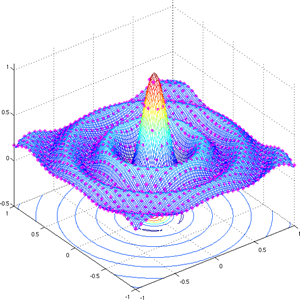
\includegraphics[scale=0.25]{../../img/sinc.PNG}}
考虑 \(N_{T}\times N_{R}\) 天线配置的MIMO-OFDM系统,子载波数目为 \(K\) , \(T\) 为系统的采样时间间隔, \(B=1/T\) 为系统带宽, \(N_g\) 为循环前缀的长度,通常 \(K\gg N_g\) ,则OFDM符号周期为 \(T_s=(K+N_g)T=N_sT\) 。假定理想的时间同步,各天线之间有相同的延时功率谱,多径数目为 \(L\) ,同时 \(N_g \ge L-1\)  以避免ISI,此时 \(T_s \gg LT\) ,表明系统的子载波带宽远远小于信道的相干带宽,则 \(n\) 时刻第 \(i\) 接收天线上的食欲基带接收信号为:
\begin{equation}
  \label{eq:rxsignal}
  r_i(n) = \sum_{j=1}^{N_T}\sum_{l=0}^{L-1} h_{ij}(n,l)u_j(n-l) + \omega_i(n),\quad 1\le i \le N_R, -\infty \le n\le +\infty
\end{equation}
其中, \(h_{ij}(n,l)\) 表示 \(n\) 时刻第 \(j\) 发射天线到第 \(i\) 接收天线之间第 \(l\) 径信道衰落。 \(u_j(n)\) 为第 \(j\)  条天线上的基带发送信号; \(\omega_i(n)\) 为 \(n\) 时刻第 \(i\) 接收天线上的加性高斯白噪声,方差为 \(\sigma_{\omega}^2\) 。多天线发射信号,接收信号和噪声可以写成矢量形式:
\begin{eqnarray}
  \pmb{u}(n) &=& [u_1(n), u_2(n), \dots, u_{N_T}(n)]^T \nonumber \\
  \pmb{r}(n) &=& [r_1(n), r_2(n), \dots, r_{N_R}(n)]^T \nonumber \\
  \pmb{\omega}(n) &=& [\omega_1(n), \omega_2(n), \dots, \omega_{N_R}(n)]^T \nonumber
\end{eqnarray}
第 \(n\) 个OFDM符号时刻的接收信号可以标示为:
\begin{equation}
  \label{eq:nofdm}
  \tilde{\pmb{r}}(n) = \tilde{\pmb{H}}\tilde{\pmb{u}}(n) + \tilde{\omega} (n)
\end{equation}
其中:
\begin{eqnarray}
  \tilde{\pmb{r}}(n) &=&
  \begin{pmatrix}
    \pmb{r}(nN_s +N_g) \\
    \vdots \\
    \pmb{r}(nN_s +N_s - 1)
  \end{pmatrix}     \nonumber \\
    \tilde{\pmb{u}}(n) &=&
  \begin{pmatrix}
    \pmb{u}(nN_s +N_g) \\
    \vdots \\
    \pmb{u}(nN_s +N_s - 1)
  \end{pmatrix}     \nonumber \\
    \tilde{\pmb{\omega}}(n) &=&
  \begin{pmatrix}
    \pmb{\omega}(nN_s +N_g) \\
    \vdots \\
    \pmb{\omega}(nN_s +N_s - 1)
  \end{pmatrix}     \nonumber \\
   \tilde{\pmb{u}}(n) &=& (\pmb{F}^{-1} \otimes \pmb{I}_{N_T}) \pmb{x}(n) \nonumber
\end{eqnarray}
\(\otimes\)  是Kronecker积, \(\pmb{x}(n)\) 是 \(n\) 时刻的频域多天线发射信号, \(\widetilde{\pmb{H}}\) 是 \(KN_{R} \times KN_T\) 维的块循环矩阵。
\begin{equation}
  \label{eq:channelH}
  \widetilde{\pmb{{H}}} =\\
  \begin{bmatrix}
    \pmb{G}(0)    &  \pmb{0}_{N_RN_T}  & \cdots                         &  \pmb{0}_{N_RN_T}  & \pmb{G}(L-1)         &\cdots                       & \pmb{G}(1)      \\
   \pmb{G}(1)     &  \pmb{G}(0)             & \pmb{0}_{N_RN_T}  &  \cdots                        & \pmb{0}_{N_RN_T}   & \ddots                      & \vdots                \\
    \vdots                &  \ddots                        &  \ddots                        & \pmb{0}_{N_RN_T}   & \cdots                          &\pmb{0}_{N_RN_T} & \pmb{G}(L-1) \\
   \pmb{G}(L-1) &   \cdots                       &\pmb{G}(1)               &\pmb{G}(0)             & \pmb{0}_{N_RN_T}    & \cdots                      &\pmb{0}_{N_RN_T}\\
\pmb{0}_{N_RN_T}& \ddots                       & \cdots                        & \ddots                         &\ddots                           & \ddots                      & \vdots                 \\
 \vdots                    & \ddots                       &\ddots                            & \cdots                        &\ddots                          &\pmb{G}(0)           &\pmb{0}_{N_RN_T}\\
\pmb{0}_{N_RN_T}& \cdots                      &\pmb{0}_{N_RN_T}   & \pmb{G}(L-1)           &\cdots                           &\pmb{G}(1)          & \pmb{G}(0)
  \end{bmatrix}
\end{equation}
\(\pmb{ G}(l)\) 为收发天线阵之间第 \(l\) 径信道矩阵,其维数为 \(N_R\times N_T\) ,
\begin{equation}
  \label{eq:20120319gl}
  \pmb{G}(l) =
  \begin{bmatrix}
    h_{11}(l) & h_{12}(l) & \cdots & h_{1N_T} \\
    h_{21}(l) & H_{22}(l) & \cdots & h_{2N_T} \\
    \vdots  & \vdots     & \ddots  &\vdots   \\
    h_{N_R1} & \cdots & \cdots & h_{N_RN_T}(l)
  \end{bmatrix}
\end{equation}
则FFT变换后的频域接收信号为:
\begin{eqnarray}
  \label{eq:20120319yn}
  \pmb{y}(n) &=& (\pmb{F}\otimes \pmb{(I)}_{N_R}) \tilde{\pmb{r}}(n) \nonumber \\
                        &=& (\pmb{F}\otimes \pmb{I}_{N_R}) (\tilde{\pmb{H}}\tilde{\pmb{u}}(n) + \tilde{\omega} (n)) \nonumber \\
                        &=& (\pmb{F}\otimes \pmb{I}_{N_R}) (\tilde{\pmb{H}}(\pmb{F}^{-1} \otimes \pmb{I}_{N_T}) \pmb{x}(n) + \tilde{\pmb{\omega}}(n))   \nonumber \\
                        &=&  (\pmb{F}\otimes \pmb{I}_{N_R}) \tilde{\pmb{H}}(\pmb{F}^{-1} \otimes \pmb{I}_{N_T}) \pmb{x}(n) + \pmb{z}(n)
\end{eqnarray}
令 \$\pmb{U}\_\{DFT\} = \pmb{F}\(\otimes\) \pmb{I}\_\{N\_R\}) \$ , \$\pmb{U}\_\{DFT\}\^{}\{-1\}= \pmb{F}\^{}\{-1\}\(\otimes\) \pmb{I}\_\{N\_T\}) \$ ,则它们都是酉矩阵。 \(\pmb{F}\) 为傅里叶变换矩阵,记 \(W_{K}^{kl} = e^{-j2\pi kl/K}\) ,则 \(\pmb{F}\) 可以标示如下:
\begin{equation}
  \label{eq:20120319f}
  \pmb{F} =
  \begin{bmatrix}
  1&  1                &    \cdots  &  1 \\
  1&  W_{K}^1     &     \cdots &  W_{K}^{K-1}  \\
   \vdots & \vdots & \ddots & \vdots \\
   1& W_{K}^{K-1}  & \cdots  &   W_{K}^{(K-1)(K-1)}
  \end{bmatrix}
\end{equation}
利用分块矩阵的特点以及循环矩阵可以对角化的定理,
\begin{equation}
  \label{eq:20120319uhu}
  \pmb{U}_{DFT} \tilde{\pmb{H}} \pmb{U}_{DFT}^{-1} = \pmb{\Lambda}
\end{equation}
\begin{equation}
  \label{eq:20120319diag}
  diag{\pmb{\Lambda_{k}}} = \sum_{l=0}^{L-1} \pmb{G}(l) e^{-j2\pi kl/K}
\end{equation}
这里有一个疑问,式\textasciitilde{}(\ref{eq:20120319diag})右边最后一个因子 \(e^{-j2\pi kl/K}\) 不确定。根据以上可以得到:
\begin{equation}
  \label{eq:20120319yn2}
  \pmb{y}(n) = \pmb{\Lambda}\pmb{x}(n) + \pmb{z}(n)
\end{equation}
其中, \(\pmb{z}(n)\) 为频域噪声矢量,由于DFT是酉变换,不改变噪声的统计特性, \(\pmb{z}(n)\) 中个元素仍然满足独立同分布的高斯分布。  \(\pmb{\Lambda}\) 为分块对角矩阵。
\begin{equation}
  \label{eq:20120319lamda}
  \pmb{\Lambda} =
  \begin{bmatrix}
    \pmb{H}(n,0) & \cdots & 0 \\
    \vdots                &     \ddots & \vdots \\
    0                         & \cdots   & \pmb{H}(n,K-1)
  \end{bmatrix}
\end{equation}
\begin{equation}
  \label{eq:20120319hnk}
  \pmb{H}(n,k) =
  \begin{bmatrix}
    H_{11}(n,k)   &  H_{12}(n,k) & \cdots   & H_{1N_T}(n,k) \\
    H_{21}(n,k)   &  H_{22}(n,k) &  \cdots &  H_{2N_T}(n,k) \\
    \vdots          & \vdots          &\ddots &   \vdots  \\
    H_{N_R1}(n,k) & \cdots         &\cdots &  H_{N_RN_T}(n,k)
  \end{bmatrix}
\end{equation}
则 \(n\) 时刻子载波 \(k\) 上的接收信号可表示为:
\begin{equation}
  \label{eq:20120319yink}
 y_i(n,k) = \sum_{j=1}^{N_T} H_{ij}(n,k)x_j(n,k) + z(n,k)
\end{equation}
写成矢量形式为:
\begin{equation}
  \label{eq:20120319yinkvcetor}
  \pmb{y}(n,k) =\pmb{H}(n,k)\pmb{x}(n,k) + \pmb{z}(n,k)
\end{equation}
其中 \(\pmb{H}(n,k)\)  中的元素 \(H_{ij}(n,k)\) 为 \(n\) 时刻在第 \(k\) 子载波上对应的第 \(j\) 发送天线到第 \(i\) 接收天线频率响应:
\begin{equation}
  \label{eq:20120319hijnk}
  H_{ij}(n,k) = \sum_{l=0}^{L-1} h_{ij}(n,l) W_{K}^{kl}
\end{equation}
第 \(j\) 发送天线到第 \(i\) 接收天线对之间的 \(L\) 径时域信道响应可写成矢量形式:
\begin{equation}
  \mathbf{h}_{ij} = [h_{ij}(n,0), h_{ij}(n,1), ..., h_{ij}(n,L-1)]^T \qquad 1 < i < N_R, 1 < j < N_T
\end{equation}
\end{document}
